\documentclass{standalone}
\usepackage{graphicx}	
\usepackage{amssymb, amsmath}
\usepackage{color}

\usepackage{tikz}
\usetikzlibrary{calc, arrows.meta}
\usepackage{pgfmath}

\definecolor{light}{RGB}{220, 188, 188}
\definecolor{mid}{RGB}{185, 124, 124}
\definecolor{dark}{RGB}{143, 39, 39}
\definecolor{highlight}{RGB}{180, 31, 180}
\definecolor{gray10}{gray}{0.1}
\definecolor{gray20}{gray}{0.2}
\definecolor{gray30}{gray}{0.3}
\definecolor{gray40}{gray}{0.4}
\definecolor{gray60}{gray}{0.6}
\definecolor{gray70}{gray}{0.7}
\definecolor{gray80}{gray}{0.8}
\definecolor{gray90}{gray}{0.9}
\definecolor{gray95}{gray}{0.95}

\newcommand*{\offset}{0.025}

\begin{document}

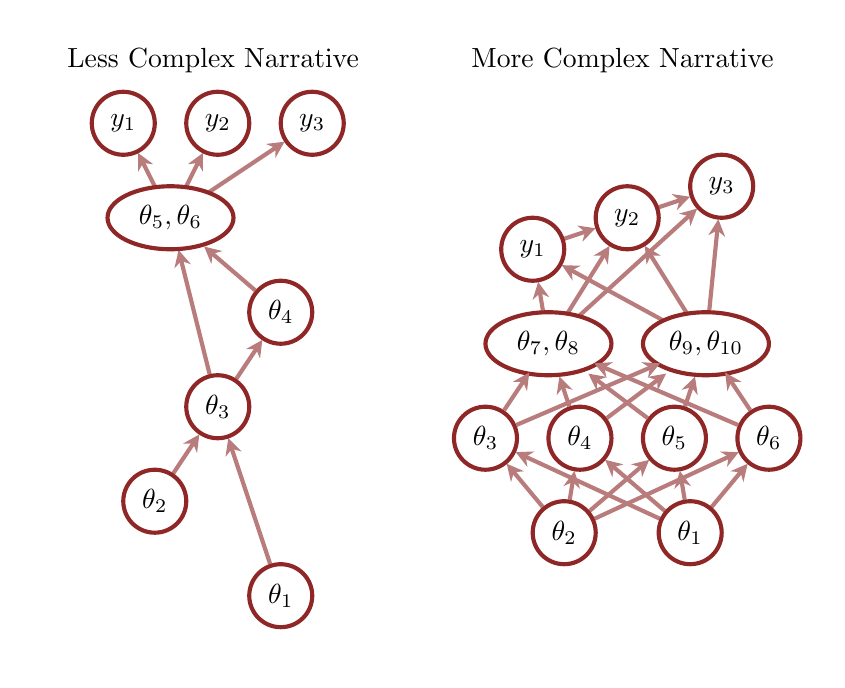
\begin{tikzpicture}[scale=0.2, thick]

  \pgfmathsetmacro{\r}{2}
    
  \begin{scope}[shift={(0, 0)}]
    \draw[white] (-12, -4) rectangle (12, 36);
  
    \node[align=center] at (0, 34) { Less Complex Narrative };
  
    \coordinate (A) at (4, 0);
    \coordinate (B) at (-4, 6);
    \coordinate (C) at (0, 12);
    \coordinate (D) at (4, 18);
    \coordinate (E) at (-3, 24);
    \coordinate (F) at (-6, 30);
    \coordinate (G) at (0, 30);
    \coordinate (H) at (6, 30);

    \foreach \B/\E in {A/C, B/C, C/D, C/E, E/F, E/G, E/H} {
      \draw[-{Stealth[length=6pt, width=6pt]}, shorten <=12.1, shorten >=12, color=mid, line width=1.5] (\B) -- (\E);
    }

    \filldraw[fill=white, draw=dark, line width=1.5] (A) circle (\r)
    node[color=black] { $\theta_{1}$ };

    \filldraw[fill=white, draw=dark, line width=1.5] (B) circle (\r)
    node[color=black] { $\theta_{2}$ };

    \filldraw[fill=white, draw=dark, line width=1.5] (C) circle (\r)
    node[color=black] { $\theta_{3}$ };
    
    \filldraw[fill=white, draw=dark, line width=1.5] (D) circle (\r)
    node[color=black] { $\theta_{4}$ };
    
    \filldraw[fill=white, draw=dark, line width=1.5] (E) circle [x radius={2 * \r}, y radius={\r}]
    node[color=black] { $\theta_{5}, \theta_{6}$ };
    
    \filldraw[fill=white, draw=dark, line width=1.5] (F) circle (\r)
    node[color=black] { $y_{1}$ };
      
    \filldraw[fill=white, draw=dark, line width=1.5] (G) circle (\r)
    node[color=black] { $y_{2}$ };

    \filldraw[fill=white, draw=dark, line width=1.5] (H) circle (\r)
    node[color=black] { $y_{3}$ };

    \foreach \B/\E in {D/E} {
      \draw[-{Stealth[length=6pt, width=6pt]}, shorten <=12.1, shorten >=16, color=mid, line width=1.5] (\B) -- (\E);
    }

  \end{scope}

  \begin{scope}[shift={(26, 0)}]
    \draw[white] (-12, -4) rectangle (12, 36);
  
    \node[align=center] at (0, 34) { More Complex Narrative };
  
    \coordinate (A) at (4, 4);
    \coordinate (B) at (-4, 4);
    \coordinate (C) at (-9, 10);
    \coordinate (D) at (-3, 10);
    \coordinate (E) at (+3, 10);
    \coordinate (F) at (+9, 10);
    \coordinate (G) at (-5, 16);
    \coordinate (H) at (5, 16);
    \coordinate (I) at (-6, 22);
    \coordinate (J) at (0, 24);
    \coordinate (K) at (+6, 26);

    \foreach \B/\E in {A/C, A/D, A/E, A/F, B/C, B/D, B/E, B/F, G/I, G/J, G/K, H/I, H/J, H/K, I/J, J/K} {
      \draw[-{Stealth[length=6pt, width=6pt]}, shorten <=12.1, shorten >=12, color=mid, line width=1.5] (\B) -- (\E);
    }

    \filldraw[fill=white, draw=dark, line width=1.5] (A) circle (\r)
    node[color=black] { $\theta_{1}$ };

    \filldraw[fill=white, draw=dark, line width=1.5] (B) circle (\r)
    node[color=black] { $\theta_{2}$ };

    \filldraw[fill=white, draw=dark, line width=1.5] (C) circle (\r)
    node[color=black] { $\theta_{3}$ };
    
    \filldraw[fill=white, draw=dark, line width=1.5] (D) circle (\r)
    node[color=black] { $\theta_{4}$ };

    \filldraw[fill=white, draw=dark, line width=1.5] (E) circle (\r)
    node[color=black] { $\theta_{5}$ };
    
    \filldraw[fill=white, draw=dark, line width=1.5] (F) circle (\r)
    node[color=black] { $\theta_{6}$ };
    
    \filldraw[fill=white, draw=dark, line width=1.5] (G) circle [x radius={2 * \r}, y radius={\r}]
    node[color=black] { $\theta_{7}, \theta_{8}$ };

    \filldraw[fill=white, draw=dark, line width=1.5] (H) circle [x radius={2 * \r}, y radius={\r}]
    node[color=black] { $\theta_{9}, \theta_{10}$ };

    \filldraw[fill=white, draw=dark, line width=1.5] (I) circle (\r)
    node[color=black] { $y_{1}$ };
      
    \filldraw[fill=white, draw=dark, line width=1.5] (J) circle (\r)
    node[color=black] { $y_{2}$ };

    \filldraw[fill=white, draw=dark, line width=1.5] (K) circle (\r)
    node[color=black] { $y_{3}$ };

    \foreach \B/\E in {E/G, F/G, C/H, D/H} {
      \draw[-{Stealth[length=6pt, width=6pt]}, shorten <=12.1, shorten >=18, color=mid, line width=1.5] (\B) -- (\E);
    }

    \foreach \B/\E in {C/G, D/G, E/H, F/H} {
      \draw[-{Stealth[length=6pt, width=6pt]}, shorten <=12.1, shorten >=12.5, color=mid, line width=1.5] (\B) -- (\E);
    }

  \end{scope}

\end{tikzpicture}

\end{document}  